\documentclass[a4paper]{article}

\usepackage{amsmath}
\usepackage[margin=2.5cm]{geometry}
\usepackage{listings, listings-rust}
\usepackage{graphicx}
\usepackage{wrapfig}

\newcommand\figref[1]{Figure~\ref{#1}}

\title{OTP in Rust}
\author{Andreas Nicolaisen - \texttt{jtc313} \\ Marco Aslak Persson - \texttt{bfr555}}
\date{\today}

\begin{document}

% TODO: Actors vs. processes

\maketitle

\section{Introduction}

\section{Background \& Analysis}
%% \textit{What's OTP?}
%% \begin{itemize}
%% \item What is the actor model
%% \item What is the goal of OTP?
%% \item What are the ``design principles'' of OTP?
%% \item How is it used?
%% \end{itemize}

%% \textit{How does this interact with Erlang}
%% \begin{itemize}
%% \item What parts of Erlang/BEAM is ``needed'' for implementing OTP? (processes,
%%   traps, mailboxes \& etc.)
%% \end{itemize}

%% \textit{Will probably have a similar structure to the Suture blog-post}
%% \begin{itemize}
%% \item What parts of OTP are we interested in porting.
%% \item How does this translate to Rust?
%% \item What does Rust make easier/harder?
%% \item What different things could an implementation focus on?
%%   \textit{Like performance, robustness, idiomaticity, expressiveness, ergonomics}.

%%   We'll try to find out whether it \textit{can} be done idiomaticly and ergonomically.

%% \item What have we chosen to focus on?
%% \end{itemize}

%% An implementation of an OTP-alike library will have to contain functionality in the lines of:
%% \begin{itemize}
%% \item \textbf{Message sending}\\
%%   The different actors should be able to communicate with each others, using
%%   messages. To accomplish this, they will need some way to refer to each other.
%%   This could be done by using global ids, registered names or passing around
%%   references to each other.
%% \item \textbf{Supervisor trees}\\
%%   In order to organize the program, the actors should be organized into
%%   supervisor trees. These will be trees of supervisor actors, with worker actors
%%   as leafes. The supervisors should be able to monitor and restart its children,
%%   should they crash, in accordance with supplied strategies and policies.
%% \item \textbf{Behaviours}
%% \end{itemize}

% TODO: Talk about local and global naming

\subsection{The actor model}
In the actor model, an application is structured around a collections of
independent actors. Generally, each actor has the following abilities:
\begin{itemize}
\item Each actor has the abiltity to send messages to other actors, and
  themselves receive messages.
\item The actors can decide to take any action they desire based, on the messages
  they receive. This includes modifying some state that they hold on to, which
  can then be used when responding to later messages.
\item Each actor can spawn new actors.
\end{itemize}

The actors exist as seperate entities, and should not be able to affect each
other, unless it is through messaging each other. Typically, a lot of actors are
created, and each actor is tasked with handeling small tasks.\\

\noindent
The message passing itself can be realized in two different ways, synchronous
and asynchronous. By synchronous, it is understood that when an actors sends
another actor a message, it will only continue its execution when the other
actor has received the message. By asynchronous, it is understood that the
message is sent much like a letter, in that once we have sent a message we don't
know when/if the other actor will receive it. In different realizations of the
actor model, there will be different guarantees as to whether messages will
always be received, or if they can be lost, as well as what order the messages
can be in. How the message passing works will also differ. All actors might have
some address that can be used to send them messages, or be given names that can
change what they refer to, during the execution of the program.

\subsection{Erlang processes}
As mentioned, in an idiomatic actor model system, a lot of actors are often
created. This means that we have the possibility to run the actors concurrently,
but we have to be careful of how we do it. If we were to fx. run each actor on a
seperate OS thread, we would encounter a large overhead each time a new actor
are created (as well as the cost of context switching). Erlang solves this by
providing lightweight processes, which are quick to create and only take up a
small amount of memory when created.\\

\noindent This allows us to use a new process for each actor that we want in our
system, without encountering a large overhead. Each process is equipped with a
\texttt{PID} (Process IDentifer). If an process (or actor) knows another's PID,
they can use it to send them messages, monitor it, as well as ``kill'' it.
Message sending is asynchronous, and anything can be sent. The other process can
then specify what it want to receive at a given time, and how to act based upon
the messages it receives. By monitoring another process, the monitoring process
will be notified if the monitored processs dies\footnote{Processes can also link
to each other, but that is beyond the scope if this project}. While this is not
part of the actor model, it is often quite useful. By sending a special signal,
a process can ``kill'' another process, which shutdowns the process, no matter
what is was currently doing. This is useful when organizing actors in
\textit{supervision trees}, which will be discussed in the next section.

\subsection{OTP}
Developing application with Erlang is most often coupled with using OTP (Open
Telecom Platform). OTP is a platform consisting of a compiler, libraries,
middelwares, a database and some tools. What we will be most concerned with is
supervision trees and behaviors.

\subsubsection{Supervision trees}
Supervision trees are a way to organize actors into supervisors and workers, in
a way that supports reliability. This is under the philosophy that parts of any
implementation will, from time to time, crash, and it should be setup to handle
it when it does. An example of a supervision tree can be seen in
\figref{fig:supervision_tree}.

\begin{figure}[h]
  \centering
  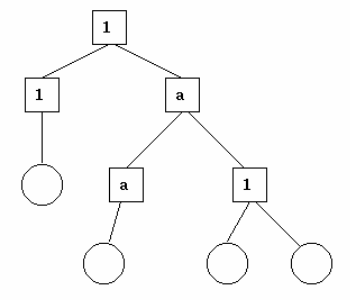
\includegraphics[width=0.5\textwidth]{./resources/SupervisionTree.png}
  \caption{An example of a supervision tree, the square nodes are supervisors,
    and the round nodes are workers} % TODO: source:  https://erlang.org/doc/design_principles/des_princ.html#supervision-trees 
  \label{fig:supervision_tree}
\end{figure}

\noindent
A supervisor will have a number of children, which can be both workers and other
supervisors. Should any of a supervisor's children shutdown unexpectedly, the
supervisor have the responsibility of starting it back up again, if it is
specified that it should be restarted. Further, the children could have
interdepencies, so the supervisors can also restart other children than the ones
who shutdown unexpectedly.

\subsubsection{Behaviors}
In an actor model system, many actors will often follow similar patterns. For
example, all of the supervisors in a tree will follow a similar patterns, some
actors will be simple servers, some will be state machines, etc. Knowing this,
OTP providers modules for a number of behaviors. These split the implementation
of the actor into 2 parts, the generic part and part specific to the actor. The
generic part is implemented in OTP, and the part specific to the actor is left
for the user to implement. This is done by implementing a set of callback
functions. These are used by the generic part of the behavior, and is where the
user implements their part of the actor.

\subsection{How can this be implemented in Rust}
\begin{itemize}
\item \textbf{Immutability and actor isolation}\\
  In Erlang all data are imutable, and processes are isolated from each other.
  One of the main benefits of isolation, is to avoid shared mutable state, and
  the problems the arise from. In Rust, different threads are not isolated from
  each other the same way that processes in Erlang are, and neither are all data
  immutable. However, Rusts type system prevents the danger of mutable shared
  state, both in single and multi thread contexts, avoiding the common downsides
  of shared and mutable state. This means that the actors can affect other
  threads by ways other than message passing, however, the common downsides of
  this are avoided.
\item \textbf{Message passing}\\
  Unlike in Erlang, there are no intrinsics for sending and receiving messages
  in Rust. However, the standard library provides a multiple producer, single
  comsumer channel which fulfills this purpose. It will require some more code
  to create and handle these channels, but hopefully this can all be done in the
  library itself, so that the experience of messaging other actors are largely
  the same as in Erlang.
\item \textbf{Monitoring and killing other processes}\\
  We have chosen to realize our actors as tokio tasks (see design/implementation
  sections), which does not provide the same functionality as Erlang does for
  its processes.

  This means that we cannot simply monitor other actors the way we can in
  Erlang. We \textit{can} know when a task finishes, but only by awaiting its
  joinhandle, which can only be done by one thread. This is becaused it cannot
  be cloned. This means that we need to implement some system for notifying
  other actors, of when an actor terminates, inorder to get the same monitoring
  functionality.

  We cannot kill other tasks the same way we can in Erlang, and this is one of
  the points where our library is going to differ from Erlang/OTP. This could
  theoretically be done if we were using OS threads, but for reasons discussed
  in the design section, we're not. Instead, we allow for asking another actor
  to terminate itself, by sending a message. These kinds of messages are
  prioritised over other kinds of messages, so it achevives close to the same
  semantics are Erlang, but not exactly.
\item \textbf{Behaviors}\\
  In Erlang/OTP, the way you use behaviors, is by implementing a set of callback
  functions, which are then called by the behavior module. The way to do this in
  Rust is to implement a trait, with a series of methods, for a type. These
  accomplish the same thing, using different language features.
\end{itemize}

\section{Design}
%% \begin{itemize}
%% \item Talk about what an OTP implementation overall consists of (in general)
%% \item Talk about our high-level design decisions
%% \item Talk about what design experiments we did (And explain why we went back on
%%   some of them)
%% \end{itemize}
\subsection{Design goals}
In the design of our library, we have set the following goals:
\begin{itemize}
\item Implement an OTP-like (or rather, a subset of it) system in Rust in a way
  that is idiomatic to Rust.
\item Strongly type the messages that the actors will pass to each other.
\item Allow the user to write idiomatic actor model code, in a way that is also
  idiomatic to Rust.
\item Enable to user to easily organize their actors in supervisor trees, both
  in a declarative as well as dynamic fashion.
\item Make it easy for the user to implement common patterns, without having to
  worry about how the actors interacts with the supervision tree.
\end{itemize}

\noindent
Overall, the aim is to create a library that provides better type-safety than
what is experienced in Erlang, without making it harder to implement an
application. This should be accomblished by using Rust's own guarantees, so that
a programmer experienced with Rust can use it, without a large barrier to entry.

\subsection{Design details}
We've designed our library to be implemented with an asynchronous execution
model. This allows us to easily acheive concurrency between the actors, in both
single and multi-threaded contexts. It is not necessarily a requirement for
actors to run in parallel. By making our library asynchronous we enable the
implementation to take advantage of cooperative multi-threading via ``green
threads'', which can both work in single-threaded and multi-threaded contexts.
Green threads are a more light-weight alternative to using operating system
threads, which is important because idiomatic use of the actor model often
involves creating actors for even small tasks. If creating an actor required
starting an operating system thread, then the overhead would be quite signficant
compared to green threads.\\

% What is actor?
\noindent
Actors in our library are realized as isolated computations % ?: Word choice
which receive and acts upon messages sent to them through their mailboxes.\\

\noindent
Mailboxes are objects that enables the sending of messages to an actor, and are
comparable to PIDs in Erlang. We've opted to not hide mailboxes behind an
indirection, like a PID, and instead make actors use and store the
data-structure required for the actual sending of message directly. This is done
to avoid having to do extra book-keeping (like maintaining a --- possibly global
--- map of PID to the data-structure required for sending message). This is at
the cost of having to possibly store more data per mailbox compared to PID, as
well as having to clone the mailbox whenever it needs to be sent to another
actor (which is required due to Rust's ownership system).\\

\noindent
All actors can receive two kinds of messages. The first being system messages
which pertain to system-level concerns. Currently this only involves requesting
an actor to shut down. In addition to system messages, actors can also
receive messages of their own specific message type. The message type of an
actor is specified as part of the actor's implementation. The only requirement
for an actor's message type is that it's transferable between threads, i.e. it
implements/satisfies the \texttt{Send} trait in Rust. This requirement allows
actors to run on seperate threads. Though by only having this requirement, we do
not have the required invariants to allow for inter-process or remote
communication between actors, since that would require that messages were also
serializable. The reason we choose to have the system messages as a seperate
thing, is to make it easier to deal with actors of different types, in contexts
where their type is irrelevant (such as in the supervisor implementaiton). In
hindsight, this is properly an unnecesarry complication, since all messages
could be wrapped in an some sort of \texttt{Either<SystemMessage, MessageType>},
or \texttt{SystemMessage} could have another variant containing the actors
message type. This would require more conversion in the background, but from the
users perspective, it whould properly be easier to use, and we wouldn't have to
store/use two channels for each mailbox. On the other hand, having the two kinds
of messages in seperate channels, makes it easier to prioritise system message,
without having to go through all pending messages.\\

\noindent
Actors are responsible for acting upon the messages they receive. This is mainly
inteded to be done through behaivors which in our library is the equivalent
concept as in OTP. In our library behaivors are realized as different traits
with methods for the user to implement their own business logic and usually a
helper function for starting actors implementing that behaivor.\\
% TODO: Introduce behaivors from Erlang in Background

\noindent
Given this context, we will explain our design of different parts, in more
specific terms:
\begin{itemize}
\item \textbf{Mailboxes}\\
  %% We have opted to statically type messages. This means that each actor can only
  %% receive messages of its data type, as well as ``System messages''. Message
  %% sending is accomplished using ``Mailboxes''. Using these actors can
  %% send the 2 kinds of messages to each other.
  There 3 kinds of mailboxes, unnamed, named and dynamic. Unnamed mailboxes are
  the main kind of mailbox, which allows the actors to send system messages and
  data messages to each other. Should the receiving actor crash, trying to send
  a message to it, using an unnamed mailbox, will result in an error. Named
  mailboxes are an indirection over unnamed mailboxes, used for sending messages
  to an actor that is registered globally with a name. These 2 first kind of
  mailboxes are typed over the message type. The dynamic mailbox is mainly used
  in situations where multiple different actor types can occur, such as when
  getting a list of a supervisors children. It can only be used for sending
  system messages, until the user tries to casts it to a concrete type. This
  allows the user to handle them without caring about the underlying message
  type.
\item \textbf{Actor naming}\\
  There are two forms of naming of actors, global and local, both given before
  the actor is started. The names are used for two different purposes, for
  differenting between actors locally, and for aquiring a reference to an actor.
  An actor can ask a supervirsor (usually its own) for a list of its children.
  The supervisor then replies with a list of its children, consisting of the
  children's names, and the children's mailboxes. These names will be the names
  that where given before the child was started (either global or local). If a
  child is not given a name, it will be assigned one by its supervisor. If a
  child is  globally named, it will additonally have its mailbox globally
  registered by  its supervisor on startup. This global registration is useful
  for commucating with often used actors, without having to acquire a reference
  to its mailbox through other means. This is how the named mailboxes work.
\item \textbf{Supervision}\\
  Our design of supervision breaks into two parts, how the user specifies it and
  how they interact with it. We have chosen to use a declarative approch when
  specifying how a supervision tree should be created, in order to aliviate the
  user from having to think about how supervision trees are built. Instead, they
  only have to think about how they want to structure their supervion
  tree/application. We allow the user to interact with the supervisors through
  messages, so that they can establish contact between actors dynamically. This
  is useful for dealing with dynamic instantiation of actors, and for discovering
  other actors in the supervision tree, without having to resort to global
  naming.
  \begin{itemize}
  \item \textbf{Supervisor - Specification}\\
    In order to make it easier for the user, supervision trees can be created
    declarativly, using a specification api. This consist of building blocks of
    supervisors and workers, which are put into a tree.
    % TODO: Insert example (diagram and code example)
    A supervisor will need some restart strategy, as well as list of child
    specications. A worker will need some restart policy, and also takes an
    starting argument. Both supervisors and workers can be named, either locally
    or globally.
  \item \textbf{Supervisor - Interaction}\\
    When interacting with a supervisor, it is important to note that supervisors
    themselves are actors, just like workers. This means that they can receive
    messages like any other actor. They can receive system messages asking them to
    shutdown, as well as requests. These requests allow other actors to ask for a
    list of the supervisors children, to ask the supervisor to start another
    child with given a specification, and allows for monitoring children i.e.
    being notified whenever a child is shutdown or restarted. All children are
    given a mailbox to their supervisor, so that they can make these requests of
    them.
  \end{itemize}
\item \textbf{Behaviours}\\
  The concept of behavious from OTP are implemented as traits, that should be
  implemented in order to fulfill the behaviour. This will consist of a number
  of methods that should be implemented, and they (the traits) will often be
  over a type. They will come with a helper method that provides the common
  boiler plate functionality (eg. the handeling of system messages). This
  method serves the same purpose as the behavoir module in Erlang. When a
  message passed to the actor is not part of the boiler plate, the behaviour
  will pass this message onto the implementation of the trait.
\item \textbf{Asynchronous exceptions}
  Unlike in Erlang, actors can't kill each other directly. Instead each
  actors can request that an other actors shuts itself down. The handeling of
  this message will then take place in library code, to avoid usercode from
  simply ignoring the request. Since the messages are handled sequentially this
  means that actors cannot be shut down when they are handeling another
  messages. This has the advantage of avoiding actors being shutdown in crital
  sections, but has the disadvantage of not being able to shutdown an actor that
  is stuck. This is the only practical way of shutting down an actor, since it
  is not possible to stop a scheduled task. One way shutting down a running
  actor \textit{could} be done, it to have each actor be its own seperate OS
  thread, which you could then ask the OS to shutdown. The comes with the
  downside mentioned earlier, of not being able to take advantage of ``green
  threads''.
\end{itemize}

\section{Implementation}
%
% Immutability (we don't really use it)
% Runtime choice
We have chosen to base our implementation on the Tokio library. Tokio provides an
asynchronous execution runtime, with support for \texttt{Task}s, which are
light-weight non-blocking execution units. This is especially useful because we
want the overhead of spawning actors to be low.
\begin{itemize}
\item{\bf Mailboxes} \\
Mailboxes are implemented as an abstraction on top of channels. Channels as a
concept are both found in the Rust standard library, and in Tokio, and they are a
mechanism for sending values between threads via a FIFO queue. Specifically, we
use the multi-producer, single-consumer (\texttt{mpsc}) kind. Such a channel
consists of a unique \texttt{Receiver}-end and any number of \texttt{Sender}s.
The actor owns the \texttt{Receiver} end and uses it to accept incoming
messages, while the \texttt{Sender}s are abstracted over as mailboxes. Normally
it is the responsibility of the library part of the behavior, to handle the
actual reception of messages. Therefore, the receiver is normally exposed to the
behavior implementer.
% - Boundedness
Tokio
provides two kinds of \texttt{mpsc} channel, bounded and unbounded. Sending
never blocks for unbounded channels, while bounded ones can only hold a
specified amount of unhandled messages. We've chosen to use bounded channels
with a capacity of 512 for our mailbox implementation. While we want message
sending to be asynchronous --- which unbounded always provide, and bounded only
does until their capacity is reached --- we've still opted for bounded channels
with a high capacity because it makes dealing with runway situation easier.
Instead of simply endlessly sending messages into to the ever-growing queue,
which could eventually hog all the device's memory, the sender is instead
(temporarily) blocked or deadlocked, which is easier to debug than a runaway
resource-consuming program.
% - bounded debugability
This choice has mainly been a development practicality choice and were we to
further develop this library, we would allow the user to specify whether they
want their mailboxes to be bounded or unbounded, and in the former case with
what capacity. This should be a relatively easy extension since the actual
choice of channel is hidden behind our mailbox abstraction.

As mentioned in the design section we have a couple of different types of
mailboxes. First of all, we have a mailbox trait (called \texttt{Mailbox}) which
allows for code be generically parametric over which specific type of mailbox it
deals with. The mailbox trait supports sending messages of the associated
message type and querying whether the mailbox has been closed. The most commonly
used mailbox type is the \texttt{UnnamedMailbox}, which simply behaves as an
abstraction over the underlying channel. The \texttt{NamedMailbox} extends the
unnamed variety with a naming indirection. While an unnamed mailbox can only be
acquired by cloning or being sent one, a named one can be acquired by resolving
a name. A global registry is maintained, mapping names to mailboxes. Operations
on a named mailbox only succeed if the name can be
resolved. If the underlying channel of the named mailbox has been closed, upon
trying to send a message via the mailbox, an attampt is made to re-resolve the name to a
mailbox of the same type. This re-resolution is done to allow for seamless
communication with a globally named actor that might have been restarted.

So far the mailboxes we've seen are parameterized over their message type. But in
some cases, we want to store mailboxes of different message types together.
Examples of such heterogeneous collections of mailboxes are the globally named
mailbox registry and supervisors' lists of children. In both cases, neither of
those perform any operations on the mailboxes that involve their message type.
In order to allow for heterogeneous storage of mailboxes, we've implemented the
\texttt{DynamicMailbox} type. It is a non-parametric mailbox which only supports
operations not involving the underlying mailbox's message type, and a method for
attempting to convert it back into a typed mailbox (which might fail if the
underlying message type doesn't match the attempted type). This means that it's
impossible to send messages of the wrong type.
It's implemented by
storing type-information about the underlying mailbox at runtime in our
\texttt{AnyBox} type, which stores the underlying mailbox in an (owned) separate
allocation, such that the layout of the \texttt{AnyBox} is homogenous, and
thereby making \texttt{DynamicMailbox}es homogenous too.
This introduces a runtime overhead on
all operations on the dynamic mailbox, but since the most common operation on
mailboxes is sending typed messages, which only can be done by converting the
dynamic mailbox into an unnamed one, this is not a big performance concern,
since that should be a relatively one-off thing in any given scenario.

\item{\bf Supervisors} \\
Supervisor trees are specified using the \texttt{SupervisorSpec} and
\texttt{ChildSpec} data-structures. \\ The \texttt{SupervisorSpec} contains the
supervisor's restart strategy (one-for-one, one-for-all or rest-for-one) and a
list of \texttt{ChildSpec}s. \texttt{ChildSpec}s contain the child's restart
policy (permanent, transient or temporary), its global or local name if any,
its type and initialization argument. \texttt{ChildSpec}s can only be
constructed using the \texttt{child} function, which is parameterized over a type
implementing the \texttt{Actor} trait and takes the policy and starting
argument. The \texttt{Actor} trait is probably poorly named since you can have
actors that don't implement it. What the \texttt{Actor} trait is responsible for
is associating a message- and argument-type with a given struct and requiring
the implementor to define a \texttt{start} method, which takes in an
initialization argument and a mailbox to the supervisor of the actor being
started (if one is present). It returns a mailbox to the newly started actor,
together with a \texttt{JoinHandle} which is the unique token used to await the
completion of the actor's task. The \texttt{child} function then fills in the
required information about the actor's type, which allows for heterogeneous
storage of different actors in the same array of \texttt{ChildSpecs} using the
same mechanism \texttt{DynamicMailbox} uses. The \texttt{ChildSpec} can then be
further annotated with either a local or global name using the \texttt{named} and
\texttt{globally\_named} methods respectively.

This technique allows us to declaratively specify a heterogeneous supervision
tree as long as all the actors in it implement the \texttt{Actor} trait.
Supervisors themselves also implement this trait, and their argument type is
their \texttt{SupervisorSpec}. When a supervisor is started, it then calls each
child's start method with their specified start argument. If supervisors are
nested, this results in a recursive depth-first initialization of the
supervisor-tree.

In a previous iteration of our supervisor implementation, we experimented with
using a single closure that had all the same responsibilities as the current
\texttt{ChildSpec}. It would take no arguments, instead possibly capturing any
arguments used for initialization. It would then be expected to
initialize, start, register the name of the actor (if any) and return the
mailbox, join-handle and restart-policy to the supervisor calling. This turned
out to be very cumbersome and prone causing type- and life-time errors due to
the nature of closures in Rust. So we instead opted for the more data-structure
oriented design, and delegated the initialization part to a more fixed scheme
described above instead of the completely free-form closure design. This not
only made specifying supervisor trees technically easier, it also made the
specifications much more readable.

The supervisor actor is implemented as an actor that handles
requests for operations like listing children, starting new children and
allowing other actors to be notified of child restarts and shutdowns (we call it
monitoring). In addition to these external messages, supervisor actors also
await notifications about the shutdown of their children via the
\texttt{JoinHandle}. Whenever such a notification is received, it inspects
whether the shutdown was due to a panic or because the task ran to completion,
and then decides what sort of restart action (if any) it should take based on
its own restart strategy and the child's restart policy. Supervisors need to
await both incoming messages as well as join-handles at the same time, to handle
whichever comes first. Tokio has a \texttt{select!} operation that allows for
doing such a thing, but it does not allow for awaiting a dynamic amount of
join-handles (or any future for that manner) this way. In order to work
around this limitation, we start a task when starting a new child, whose only
job is to await on that child's join-handle and send the result to the
supervisor over a private channel. Then the supervisor only has to listen on a
single receiver on its own end, while many of these tasks can send their join
notifications to it.

The supervisor also keeps track of a list of ``monitors'' for each child. When a
child is shutdown or restarted, all (if any) of said child's monitors are
notified about this. When notifying about a restart, the child's new mailbox is
also sent along. A monitor is simply the \texttt{Sender} end of an \texttt{mpsc}
channel, over which \texttt{MonitorMessage}s are sent. Monitors are registered
by sending the supervisor a monitor message using the \texttt{monitor} function,
which consists of the local-id of the child to be monitored and the
\texttt{Sender} to send the notification with.

\item {\bf The request-handler behaviour} \\
  This behaviour is comparable to OTP's \texttt{gen\_server}, it allows for
  defining actors that handle requests, allowing for an immediate- or delayed
  response. The user-defined part of the behaviour is facilitated by the
  \texttt{RequestHandler} trait, which consists of two type-parameters, the
  request and response types, and two methods \texttt{init} and
  \texttt{on\_request}. The \texttt{init} method is called as the first thing
  when the request-handler's task has been spawned. Its mailbox is passed along
  in order to allow the request-handler to know its own mailbox, and possibly
  send it to other actors. The \texttt{on\_request} methods takes the
  request-message, a unique request-id and a deferred reply channel. It returns
  either a \texttt{Response::Reply} with the reply value or
  \texttt{Response::NoReply}. If \texttt{on\_request} returns with a reply,
  said reply is directly sent back to the requester. If no response is returned
  by the request-handler then the reply is deferred by storing requests in a map
  using the request-id. In order to reply to a deferred request, the request-id
  together with the reply-value should be sent over the deferred-reply channel.
  By using a channel for deferred replies instead of a call-back, queue or just
  exposing the deferred-reply map, we enable the possibility of passing the
  sender for that channel on to another actor, allowing request handlers to
  delegate the reply to someone else.

  The mechanism used for allowing requesters to get a reply back is by bundling
  their actual request-message together with the sender-end of a
  oneshot-channel. A oneshot-channel is a channel like \texttt{mpsc}, but which
  can only transfer a single value. Then the request-handler can send its
  response over the sender passed along with the request. The requester then
  receives the reply by awaiting a reply on the receiving end. This is done because
  it requires as little coupling as possible, the requester can pass on the
  receiving end onto any other actor that might wish to receive the value, and
  the request-handler can delegate the reply to any other actor as explained
  earlier. There is no need to communicate a mailbox for the request-handler to
  reply back to, which in itself would introduce challenges, since what message
  should the request-handler even reply with? That would require further
  specification. While it is possible, and might even be preferable in some
  cases, this solution makes the fewest assumptions and is therefore the most
  flexible.

\end{itemize}


\begin{itemize}
\item Talk about some concrete implementation decisions (and what drove them)
\item Go into some (few) low-level technical details that might be interesting
\item Tokio, lightweight multiprocessing, like erlang.
\end{itemize}

\newpage
\section{Example}
During our design and implementation process we've used an example application
to both guide and evaluate our design and implementation. A diagram of this can
be seem in \figref{fig:example_diagram}.
% ...

\begin{figure}[h!]
  \centering
  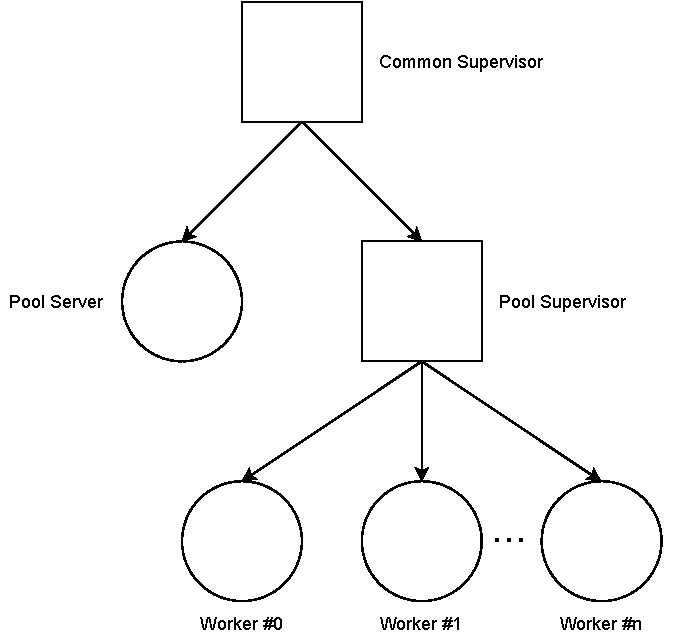
\includegraphics[width=0.5\textwidth]{./resources/PoolDiagram.pdf}
  \caption{Diagram for example}
  \label{fig:example_diagram}
\end{figure}

\begin{wrapfigure}{r}{0.4\textwidth}
\begin{lstlisting}[language=Rust,basicstyle=\footnotesize]
supervise(
  RestartStrategy::OneForAll,
  vec![
    child::<PoolServActor>
      (RestartPolicy::Permanent, ())
      .globally_named(POOL_SERV_NAME),
    supervisor(
      RestartPolicy::Permanent,
      RestartStrategy::OneForOne,
      vec![
        child::<PoolWorkerActor>
         (RestartPolicy::Permanent, ())
        ; num_workers
      ],
    ).named(POOL_SUP_NAME),
  ],
)
\end{lstlisting}
  \caption{Supervision tree specification for the example}
  \label{fig:ex-spec}
\end{wrapfigure}

The example is of a worker pool. The idea is that work can be submitted to a
work-server, which then delegates the work to a worker from the pool of workers.
The pool of workers are all transient children of the worker supervisor which
operates using a one-for-one strategy, restarting any worker that crashes. The
work-server actor and the pool-supervisor are in turn supervised under a common
supervisor. This supervisor uses the one-for-all strategy, retstarting both the
work-server and the pool-supervisor if either crashes. The specification can be
seen in \figref{fig:ex-spec}.

We have chosen this example because it is a simplified (but non-trivial) example
of an realistic application. It exercises the following aspects of our
implementation:
\begin{itemize}
\item A supervisor tree with nested supervisors
\item Supervisor interaction. The pool-server actor queries the supervisors in order
  to monitor and acquire the mailboxes of the worker actors.
\item Communication between actors. The pool-server actor sends work to the
  worker actors, and the workers reply back with the results, which the
  pool-server actor then returns to whoever submitted the work.
\end{itemize}

The pool-server implementation (\texttt{PoolServActor}) is an instance of the
\texttt{RequestHandler} behaviour. It's mesasge type is
\texttt{PoolServMessage}.

Upon being started (i.e. when its \texttt{init} method
is called), the pool-server actor retrieves its sibling's (the pool-supervisor)
mailbox by querying its own supervisor's children with \texttt{which\_children}
and finding its sibling by its local name. Then it queries the pool-supervisor
for all its children and monitors them all, then it spawns a task for each child
that receive monitor messages, and sends a message to the pool-server's mailbox
with the monitor result (whether the child has shutodwn or restarted) via the
\texttt{{PoolServMessage::WorkerMonitor}} message. This allows monitor messages
to be handled under the pool-server's \texttt{handle\_request} method.

When a peice of work is requested to be executed, the pool-server is sent a
\texttt{PoolServMessage::Start} containing the work item. It then forwards the
work item to a worker actor together with the request-id. Which worker actor is
decided based on a round-robin scheme. A task is then spawned that awaits the
reply from the worker, and forwards it to the pool-server via the
\texttt{PoolServMessage::Result} message. When the pool-server receives a result
it then uses request-id associated with the result to reply with the result to
the sender of the work request. If the pool-server receives a
\texttt{PoolServMessage::WorkerMonitor} it either panics if a worker has
shutdown (since it is going to be restarted anyway), and if the a worker has
restarted it updates its mailbox, so it has an up-to-date mailbox for that
worker.

By delegating the receiving of the result from the worker, the pool-server can
avoid blocking in the request handler while waiting for the result. Then allows
it to handle other messages while the work is completed by a worker. It would
also be possible --- instead of awaiting a reply from the worker --- to make the
worker send the result as a message to the pool-server actor instead (acquiring
the pool-servers mailbox through name resolution, since it's globally named).
We've not opted to do that in this example, even though it's a very valid way of
implementing it. The reason is that since workers are also instances of the
\texttt{RequestHandler} trait, a oneshot channel is created for the request's
reply anyway, so we opted to use that. As mentioned in the implementation
chapter, we could also extend the \texttt{RequestHandler} to handle requests
that don't expect a reply, and in that case the alternative design would make
even more sense.

The worker actors (\texttt{PoolWorkerActor}) are very simple instances of the
\texttt{RequestHandler} behaviour. They have no state and only handles one
message; the work item message, which consists of the work data and a
request-id. Upon receiving a work-item the worker simply performs the work, and
replies back with the result and the request-id.

In this example work items are just a list of integers, and the result is the
sum of those integers, but that is not very important for this example.

% What purpose does our example serve?
% - Supervisor trees, supervisor querying, interactor communication
%


\begin{itemize}
\item High-level architecture (with nice diagrams \texttt{:)})
\item Motivation, i.e. what does this example demonstrate
\item What does this example show/what can we observe/conclude from it
\end{itemize}

\section{Evaluation}
\begin{itemize}
\item What does idiomatic Rust look like? (2 parts, the implementation of OTP
  and the usage of our library)
\item How expressive is the library?
\item How easy is it to implement common patterns, in terms of ergonomics (code
  length, complexity, etc)?
\item How easy is it to understand written code?
\end{itemize}

\section{Conclusion}

\end{document}
